\documentclass[12pt,a4paper]{article}
\usepackage{amsmath,amssymb}
\usepackage{tcolorbox}
\usepackage{xcolor}
\usepackage{listings}
\usepackage{tikz}
\usetikzlibrary{automata,positioning}
\usepackage{hyperref}
\usepackage{geometry}
\usepackage{longtable}
\usepackage{array}
\geometry{margin=1in}
\usepackage{float}

% Color definitions for severity
\definecolor{redsev}{RGB}{200,0,0}
\definecolor{orangesev}{RGB}{255,140,0}
\definecolor{greensev}{RGB}{0,128,0}
\definecolor{bluesev}{RGB}{0,100,200}

% Code listing style
\lstset{
    basicstyle=\ttfamily\small,
    breaklines=true,
    keywordstyle=\color{blue},
    commentstyle=\color{green!60!black},
    stringstyle=\color{red},
    frame=single,
    captionpos=b
}

\title{OBINexus Quantum Lattice Security Framework\\
\large Formal Specification and Governance\\
\normalsize Quantum5G and Beyond: Secure Protocols over Orthogonal Span Temporary Lattices}
\author{Nnamdi Michael Okpala}
\date{\today}
\usepackage{float}


\begin{document}

\maketitle

\begin{abstract}
This document provides a comprehensive formal specification for the OBINexus quantum lattice security framework, incorporating buffer zones, cryptic state machines, and the AuraSeal quantum-resistant hashing layer. The framework enables secure quantum communication over temporary zero-trust lattices for 6G/7G networks, with adaptive governance protocols and real-time reconfiguration capabilities. We present formal mathematical foundations, security proofs, and implementation guidelines for quantum-safe communication systems that protect against both classical and quantum adversaries while ensuring compliance with electromagnetic safety standards.
\end{abstract}

\tableofcontents
\newpage

% ====================
% 1. Introduction
% ====================
\section{Introduction}

The OBINexus quantum lattice security framework represents a paradigm shift in secure communication architecture for next-generation 6G/7G networks. Built upon principles of temporary zero-trust topology, orthogonal span lattices, and quantum field theory, this framework addresses critical security challenges in quantum-era communications.

\subsection{Core Philosophy: The Red Disciple Protocol}

\begin{tcolorbox}[colback=red!10!white,colframe=red!80!black,title=Red Disciple Protocol Mindset]
\textit{``When your lattice hits RED, this ain't about panic or chaos. Nah, it's about respect, discipline, and learning the quantum language. You don't fight the vibe — you sync with it. Be the disciple, absorb the signals, and move with the flow. This is the RED Disciple Protocol, where every quantum flicker's a lesson, not a threat. Let's vibe and thrive in the cryptic chaos.''}
\end{tcolorbox}

\subsection{Framework Overview}

The framework integrates:
\begin{itemize}
    \item \textbf{Temporary Lattice Topology}: Dynamic, zero-trust communication regions
    \item \textbf{Buffer Zones}: Temporal spaces for protocol ambiguity resolution
    \item \textbf{Cryptic State Machines}: Non-deterministic automata for adaptive security
    \item \textbf{AuraSeal Layer}: Quantum-resistant hashing and integrity verification
    \item \textbf{Governance Matrix}: Severity-based security response protocols
\end{itemize}

% ====================
% 2. Buffer Regions and Protocol State Machines
% ====================
\section{Buffer Regions \& Protocol State Machines}

\subsection{Theoretical Foundation}

Within automata theory, we distinguish between behavioral and protocol state machines. The OBINexus framework introduces a third category: cryptic state machines, which model non-deterministic behavior in quantum communication protocols.

\subsection{Buffer Zone Architecture}

Buffer regions function as temporal zones within the quantum lattice where ambiguous or transitional protocol states reside. These regions serve multiple purposes:

\begin{tcolorbox}[colback=blue!5!white,colframe=blue!75!black,title=Buffer Zone Properties]
\begin{itemize}
    \item Act as network slack spaces or queues
    \item Enable context-sensitive authentication and authorization layers
    \item Allow controlled ambiguity that resolves as the system stabilizes
    \item Integrate with lattice deformation states for dynamic protocol behavior
\end{itemize}
\end{tcolorbox}

\subsection{Mathematical Formalization}

Let $\mathcal{B}$ denote the buffer zone space, defined as:
\begin{equation}
\mathcal{B} = \{(s, t, \phi) : s \in \mathcal{S}, t \in [0, \tau], \phi \in \Phi\}
\end{equation}
where:
\begin{itemize}
    \item $\mathcal{S}$ represents the state space
    \item $t$ is the temporal parameter with maximum duration $\tau$
    \item $\Phi$ is the set of possible protocol configurations
\end{itemize}

% ====================
% 3. Grammar Anchors as Protocol State Modifiers
% ====================
\section{Grammar Anchors as Protocol State Modifiers}

\subsection{Conceptual Framework}

Grammar anchors function as implicit operators that modify protocol semantics based on context. This concept draws from natural language processing where punctuation changes meaning:

\begin{tcolorbox}[colback=green!5!white,colframe=green!75!black,title=Natural Language Analogy]
Base statement: ``Don't you know how to read''\\
With ``?'': Interrogative context $\rightarrow$ Request for information\\
With ``!'': Imperative context $\rightarrow$ Expression of frustration
\end{tcolorbox}

\subsection{Protocol Application}

In the quantum lattice context, grammar anchors modify state transitions:

\begin{equation}
\text{State}_n \xrightarrow[\text{Grammar Anchor}]{\text{Buffer Zone}} \text{State}_{n+1}
\end{equation}

The transition function $\delta$ becomes context-dependent:
\begin{equation}
\delta: \mathcal{S} \times \Sigma \times \mathcal{G} \rightarrow \mathcal{P}(\mathcal{S})
\end{equation}
where $\mathcal{G}$ represents the set of grammar anchors.

% ====================
% 4. Cryptic Protocol State Machine Formalization
% ====================
\section{Cryptic Protocol State Machine Formalization}

\subsection{Red Disciple Protocol Preamble}

\begin{tcolorbox}[colback=red!10!white,colframe=red!80!black,title=Red Disciple Preamble]
\textbf{When the lattice enters RED, the operator becomes its disciple.}
\begin{itemize}
    \item Listen to quantum fluctuations
    \item Learn patterns from ambiguity
    \item Adapt responses accordingly
\end{itemize}
This state promotes harmonization, not control.
\end{tcolorbox}

\subsection{Cryptic State Machine Definition}

A cryptic state machine is formally defined as a 7-tuple:
\begin{equation}
\mathcal{M}_{\text{cryptic}} = (Q, \Sigma, \delta, q_0, F, \mathcal{C}, \Lambda)
\end{equation}
where:
\begin{itemize}
    \item $Q$ is a finite set of states
    \item $\Sigma$ is the input alphabet
    \item $\delta: Q \times \Sigma \times \mathcal{C} \rightarrow \mathcal{P}(Q)$ is the transition function
    \item $q_0 \in Q$ is the initial state
    \item $F \subseteq Q$ is the set of accepting states
    \item $\mathcal{C}$ is the context space
    \item $\Lambda$ is the set of cyclic loops
\end{itemize}

\subsection{The Hungry State Machine Example}

\begin{figure}[h]
\centering
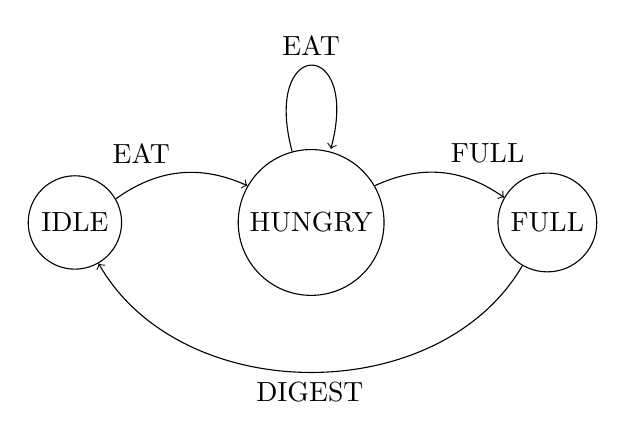
\begin{tikzpicture}[node distance=3cm,auto]
    \node[state] (idle) {IDLE};
    \node[state] (hungry) [right of=idle] {HUNGRY};
    \node[state] (full) [right of=hungry] {FULL};
    
    \path[->]
    (idle) edge[bend left] node {EAT} (hungry)
    (hungry) edge[loop above] node {EAT} (hungry)
    (hungry) edge[bend left] node {FULL} (full)
    (full) edge[bend left=60] node {DIGEST} (idle);
\end{tikzpicture}
\caption{Cryptic State Machine with Self-Loop}
\end{figure}

% ====================
% 5. AuraSeal Quantum-Resistant Hashing Layer
% ====================
\section{AuraSeal Quantum-Resistant Hashing Layer}

\subsection{Technical Architecture}

The AuraSeal layer implements a quantum-resistant cryptographic seal through the following pipeline:

\begin{tcolorbox}[colback=bluesev!10!white,colframe=bluesev!80!black,title=AuraSeal Processing Pipeline]
\begin{center}
Input Data $\rightarrow$ Salt (Dynamic Nonce) $\rightarrow$ Pre-Hash $\rightarrow$ Aura512 $\rightarrow$ \\
Quantum Distillation $\rightarrow$ Private Key Seal $\rightarrow$ Lattice Integration
\end{center}
\end{tcolorbox}

\subsection{Mathematical Specification}

\subsubsection{Pre-hashing and Salting}
\begin{equation}
h_{\text{pre}} = H_{\text{classical}}(\text{data} || \text{nonce}_{\text{session}})
\end{equation}

\subsubsection{Quantum-Distilled Hashing (Aura512)}
The quantum distillation process applies controlled noise to remove exploitable patterns:
\begin{equation}
\text{Aura512}(x) = \mathcal{D}_{\text{quantum}}\left(\sum_{i=1}^{n} \alpha_i |h_i\rangle \otimes |\psi_i\rangle\right)
\end{equation}
where $\mathcal{D}_{\text{quantum}}$ represents the distillation operator.

\subsubsection{Quantum Private Key Sealing}
\begin{equation}
\text{Seal}_{\text{final}} = \text{Sign}_{\text{QPK}}(\text{Aura512}(x))
\end{equation}

% ====================
% 6. Security Governance and Severity Levels
% ====================
\section{Security Governance and Severity Levels}

\subsection{Governance Severity Matrix}

\begin{tcolorbox}[colback=red!10!white,colframe=red!80!black,title=Critical Severity]
\textbf{Entanglement Enforcement Failure:} Full lattice compromise risk.\\
\textbf{Action:} Immediate system shutdown and quantum state collapse.
\end{tcolorbox}

\begin{tcolorbox}[colback=orangesev!10!white,colframe=orangesev!80!black,title=Warning Severity]
\textbf{Buffer Zone Quantum Activity Mismanagement:} Injection and faulty states.\\
\textbf{Action:} Review recommended before detach, enhanced monitoring.
\end{tcolorbox}

\begin{tcolorbox}[colback=greensev!10!white,colframe=greensev!80!black,title=Safe Practice]
\textbf{Grammar Anchor Integration:} Proper ambiguity handling.\\
\textbf{Action:} Continue normal operations with logging.
\end{tcolorbox}

\subsection{Error Zone Management Table}

\begin{center}
\begin{longtable}{|c|c|c|c|}
\hline
\textbf{Error Range} & \textbf{Zone} & \textbf{Severity} & \textbf{Action} \\
\hline
\endhead
0-3 & OK Zone & Safe & Detach permitted with warning \\
\hline
3-6 & Warning Zone & Elevated & Review recommended before detach \\
\hline
6-9 & Danger Zone & High & Detach not permitted - fix required \\
\hline
9-12 & Critical Zone & Critical & System panic - immediate termination \\
\hline
>12 & Extended Trace & Maximum & No-panic flag with full diagnostics \\
\hline
\end{longtable}
\end{center}

% ====================
% 7. Real-Time Lattice Reconfiguration
% ====================
\section{Real-Time Lattice Reconfiguration}

\subsection{Adaptive Topology Engine}

The lattice topology adapts in real-time based on:
\begin{enumerate}
    \item Quantum coherence measurements
    \item Network traffic patterns
    \item Security threat indicators
    \item Buffer zone occupancy
\end{enumerate}

\subsection{Reconfiguration Algorithm}

\begin{equation}
\mathcal{L}_{t+1} = \mathcal{R}(\mathcal{L}_t, \mathcal{M}_t, \mathcal{T}_t)
\end{equation}
where:
\begin{itemize}
    \item $\mathcal{L}_t$ is the lattice configuration at time $t$
    \item $\mathcal{M}_t$ represents current measurements
    \item $\mathcal{T}_t$ denotes threat assessment
    \item $\mathcal{R}$ is the reconfiguration operator
\end{itemize}

\subsection{Noise-Induced Decoherence Model}

After communication completion:
\begin{equation}
\rho_{\text{lattice}}(t > t_{\text{comm}}) = \sum_k E_k \rho_{\text{lattice}}(t_{\text{comm}}) E_k^\dagger
\end{equation}
where $E_k$ are Kraus operators representing environmental noise.

% ====================
% 8. Integration with OBINexus Toolchain
% ====================
\section{Integration with OBINexus Toolchain}

\subsection{Toolchain Architecture}

\begin{tcolorbox}[colback=gray!10!white,colframe=gray!80!black,title=OBINexus Toolchain Flow]
\texttt{riftlang.exe} $\rightarrow$ [Buffer Zone Definition] $\rightarrow$ \texttt{.so.a} $\rightarrow$ [AuraSeal Implementation] $\rightarrow$\\
\texttt{rift.exe} $\rightarrow$ [State Machine Compilation] $\rightarrow$ \texttt{gosilang} $\rightarrow$ [Protocol Deployment]
\end{tcolorbox}

\subsection{Security Hook Integration}

Each stage of the toolchain incorporates security hooks:
\begin{enumerate}
    \item \textbf{Preprocessing}: Policy enforcement and governance rules
    \item \textbf{Compilation}: Quantum byte standardization
    \item \textbf{Runtime}: Real-time lattice monitoring
    \item \textbf{Post-processing}: Decoherence verification
\end{enumerate}

\subsection{Compliance Scripts}

\begin{lstlisting}[language=bash,caption=Compliance Verification Script]
#!/bin/bash
# OBINexus Compliance Checker

echo "Verifying quantum lattice security compliance..."

# Check buffer zone configuration
verify_buffer_zones() {
    local config=$1
    # Verify temporal parameters
    # Verify state space definitions
    # Verify grammar anchor integration
}

# Validate AuraSeal implementation
check_auraseal() {
    # Verify quantum distillation
    # Check entropy thresholds
    # Validate signature schemes
}

# Main compliance loop
for module in $(find . -name "*.rift"); do
    verify_buffer_zones $module
    check_auraseal $module
done
\end{lstlisting}

% ====================
% 9. Appendix: Example State Machine Code
% ====================
\appendix
\section{Example Cryptic State Machine Implementation}

\lstset{language=C++,basicstyle=\ttfamily\small,breaklines=true}
\begin{lstlisting}[caption=Cryptic State Machine with Buffer Zones]
#include <stdio.h>
#include <quantum_lattice.h>

// Define the events
typedef enum {
    EAT,
    FULL,
    QUANTUM_FLUCTUATION
} Event;

// Define the states
typedef enum {
    IDLE,
    HUNGRY,
    FULL_STATE,
    RED_DISCIPLE  // Cryptic state
} State;

// Buffer zone structure
typedef struct {
    State current;
    float quantum_coherence;
    char grammar_anchor;
} BufferZone;

// AuraSeal verification
bool verify_auraseal(BufferZone* zone) {
    // Quantum distillation check
    if (zone->quantum_coherence < 0.25) {
        return false;  // Below entropy threshold
    }
    // Grammar anchor validation
    if (zone->grammar_anchor != '?' && 
        zone->grammar_anchor != '!') {
        return false;
    }
    return true;
}

// Cryptic state transition with buffer zones
State cryptic_transition(BufferZone* zone, Event event) {
    if (!verify_auraseal(zone)) {
        return RED_DISCIPLE;  // Enter learning mode
    }
    
    switch (zone->current) {
        case IDLE:
            if (event == EAT) {
                // Non-deterministic transition
                if (zone->quantum_coherence > 0.7) {
                    return HUNGRY;
                } else {
                    return RED_DISCIPLE;
                }
            }
            break;
            
        case HUNGRY:
            if (event == EAT) {
                // Self-loop with context
                return (zone->grammar_anchor == '?') ? 
                       HUNGRY : FULL_STATE;
            }
            break;
            
        case RED_DISCIPLE:
            // Learn from quantum fluctuations
            if (event == QUANTUM_FLUCTUATION) {
                // Harmonize with the system
                return IDLE;
            }
            break;
    }
    
    return zone->current;
}

int main() {
    BufferZone zone = {
        .current = IDLE,
        .quantum_coherence = 0.8,
        .grammar_anchor = '?'
    };
    
    printf("OBINexus Cryptic State Machine\n");
    printf("Initial state: IDLE\n");
    
    // Simulate quantum lattice communication
    while (1) {
        Event event;
        printf("Enter event (0=EAT, 1=FULL, 2=QUANTUM): ");
        scanf("%d", &event);
        
        // Update quantum coherence (simulated)
        zone.quantum_coherence *= 0.95;
        
        State next = cryptic_transition(&zone, event);
        
        if (next == RED_DISCIPLE) {
            printf("Entering RED DISCIPLE mode...\n");
            printf("Listen, learn, harmonize.\n");
        }
        
        zone.current = next;
        printf("Current state: %d, Coherence: %.2f\n", 
               zone.current, zone.quantum_coherence);
        
        // Check for decoherence
        if (zone.quantum_coherence < 0.1) {
            printf("Lattice decoherence detected.\n");
            printf("Communication session terminated.\n");
            break;
        }
    }
    
    return 0;
}
\end{lstlisting}

% ====================
% 10. Computation Matrix & QA
% ====================
\section{Computation Matrix \& Quality Assurance}

\subsection{Quantum Computation Verification Matrix}

\begin{center}
\begin{tabular}{|l|c|c|c|}
\hline
\textbf{Component} & \textbf{Classical Test} & \textbf{Quantum Test} & \textbf{Hybrid Mode} \\
\hline
Buffer Zones & Unit tests & Coherence measurement & Fuzzing \\
Grammar Anchors & Parse validation & Context entropy & State coverage \\
AuraSeal & Hash collision & Quantum resistance & Side-channel \\
Lattice Topology & Graph connectivity & Entanglement verify & Decoherence rate \\
\hline
\end{tabular}
\end{center}

\subsection{Test Case Examples}

\begin{tcolorbox}[colback=yellow!10!white,colframe=yellow!80!black,title=QA Test Suite]
\begin{enumerate}
    \item \textbf{Buffer Zone Overflow}: Verify graceful degradation
    \item \textbf{Grammar Anchor Injection}: Test for malicious modifiers
    \item \textbf{Quantum State Collapse}: Ensure proper cleanup
    \item \textbf{Lattice Persistence}: Verify no residual quantum fields
\end{enumerate}
\end{tcolorbox}

% ====================
% References
% ====================
\section*{References}

\begin{enumerate}
    \item Okpala, N. M. (2025). \textit{Formal Proofs for Confion: Post-Quantum HACC System}. OBINexus Computing.
    
    \item Okpala, N. M. (2025). \textit{The RIFT Architecture: Quantum Determinism Through Governed Computation}. OBINexus Project.
    
    \item Okpala, N. M. (2025). \textit{$\Psi$-QFT: The Wavefunction Glue - A Foundational Framework for Adaptive Evolution Beyond Dark Matter}. OBINexus Technical Specification.
    
    \item Okpala, N. M. (2025). \textit{OBINexus Cryptographic Interoperability Standard v1.0}. OBINexus Computing.
    
    \item Dirac, P. A. M. (1930). \textit{The Principles of Quantum Mechanics}. Oxford University Press.
    
    \item Aaronson, S. (2018). \textit{The Complexity of Quantum State Verification}. Foundations of Computer Science.
\end{enumerate}

\end{document}